\documentclass{beamer}

\usepackage{amsmath}
\mode<presentation>{\usetheme{UdeA}}

%% Para referenciar a pie de slide \footcite
\usepackage[style=verbose]{biblatex}
\addbibresource{biblio.bib}
% Se debe tener en cuenta lo siguiente:
% 1. Compilar el documento con PDFLaTeX
% 2. Compilar el documento con Biber
% 3. Compilar el documento con PDFLaTeX

\usepackage{multimedia}
\usepackage{hyperref}
\usepackage{media9}

\renewbibmacro*{cite:title}{%
	\printtext[bibhyperref]{%
		\printfield[citetitle]{labeltitle}%
		\setunit{\space}%
		\printtext[parens]{\printdate}%
	}%
}


\renewcommand{\figurename}{Figura}

% Temas de interés: CambridgeUS, Madrid, PaloAlto

\title{Beamer Presentation}
\author{Seminario Investigación\\Facultad de Ingeniería}

\begin{document}
	
	\frame[plain]{\titlepage}
	
	\section{Motivation}
	
	\begin{frame}{Problem Statement}
Definición del problema.
\footcitetext{Rasmunssen05}

	
	\begin{columns}
		\begin{column}{0.45\linewidth}
			\begin{block}{Definition}
				\begin{figure}
				
\includegraphics[width=0.5\linewidth]{logos/logoUdeA}
				\caption{XXXXXXXXXXX}
			\end{figure}
			\end{block}
		\end{column}
	\begin{column}{0.45\linewidth}
		\begin{figure}
			
\includegraphics[width=0.5\linewidth]{logos/logoUdeA}
			\caption{XXXXXXXXXXX}
		\end{figure}
	\end{column}
	\end{columns}

\begin{columns}
	\begin{column}{0.45\linewidth}
		\begin{block}{Definition}
			\begin{figure}
				
\includegraphics[width=0.5\linewidth]{logos/logoUdeA}
				\caption{XXXXXXXXXXX}
			\end{figure}
		\end{block}
	\end{column}
	\begin{column}{0.45\linewidth}
		\begin{figure}
			
\includegraphics[width=0.5\linewidth]{logos/logoUdeA}
			\caption{XXXXXXXXXXX}
		\end{figure}
	\end{column}
\end{columns}

\end{frame}

\begin{frame}{Test Branch}
HOLA MUNDO! \cite{Rasmunssen05}
\end{frame}
	
	\section{Materials and Methods}
	
	\begin{frame}{PCA}
	\begin{align}
	\mathbf{z} = \mathbf{W}\mathbf{x} 
	\end{align}
	
	Hola Mundo \footcite{Rasmunssen05}\footcite{artTest}
\end{frame}

\section{Media Files}

\begin{frame}{Video on the computer}
\centering
\movie[externalviewer]{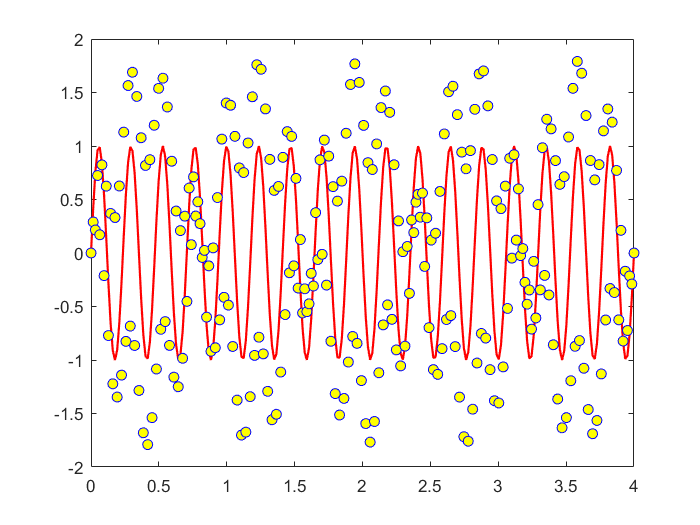
\includegraphics[width=\textheight, keepaspectratio]{img/img2}}{img/sample5s.mp4}
\end{frame}

\begin{frame}{YouTube Video}
%% see also media9 package
\begin{figure}
\centering
\href{https://youtu.be/3BLYxQKv668}{
	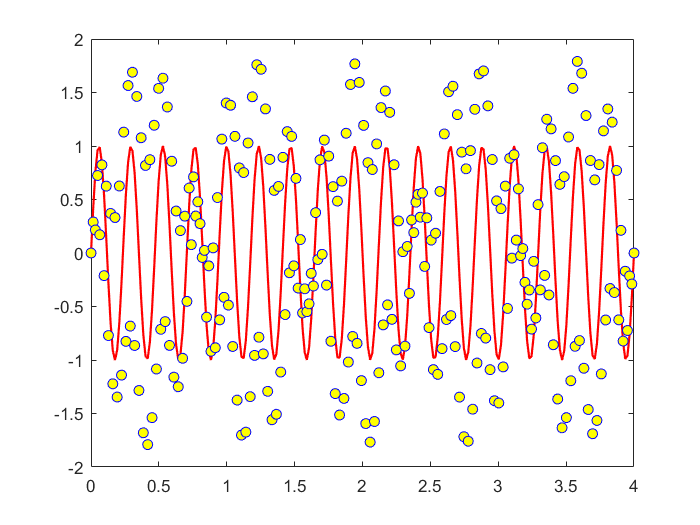
\includegraphics[width=\textheight, keepaspectratio]{img/img2}
	\label{fig:my_label}}
\end{figure}
\end{frame}

\begin{frame}{Media9 Package}
\includemedia[
width=0.6\linewidth,height=0.3375\linewidth, % 16:9
activate=pageopen,
flashvars={
	modestbranding=1 % no YT logo in control bar
	&autohide=1 % controlbar autohide
	&showinfo=0 % no title and other info before start
	&rel=0 % no related videos after end
}
]{}{http://www.youtube.com/v/r382kfkqAF4?rel=0}

\end{frame}

	\section{Results}
	
	\begin{frame}{Values}
	\begin{alertblock}{Branch alert blocks}
ALERT BLOCK!!!
	\end{alertblock}
\end{frame}
	\section{Conclusions and Future Works}
	
	\begin{frame}{Conclusions and Future Works}
\begin{itemize}
	\item Conlusion 1
	\begin{itemize}
		\item sub conclusion
	\end{itemize}
\end{itemize}
\end{frame}

\begin{frame}{REF}
%\bibliography{biblio}
%\bibliographystyle{plain}
\printbibliography
\end{frame}

\end{document}
